% Created with the help of documentation and https://www.youtube.com/watch?v=fCzF5gDy60g
% Preamble stuff
\documentclass{article} % This can be used to specify the template you will use for your document
\setlength{\parskip}{1em} % Sets the spacing between paragraphs

\usepackage[utf8]{inputenc} % Input encoding set to UTF-8 (allows emojis and stuff) (careful what compiler you use though)
\usepackage[margin=1.5in]{geometry} % Use this to specify margins
\usepackage{amsmath,amssymb} % American Math Society, allows for symbols, improves existing macros and adds for environments such as align
\usepackage{graphicx} % Allows us to embed images
\usepackage{indentfirst} % Indents the first paragraph
\usepackage{listings} % Use this for code listings
\usepackage{xcolor} % Used for styling with colors
\usepackage{array} % Used for array functionality
\usepackage{esvect} % Used for rendering vectors

\graphicspath{ {./images/} } % Sets the local folder to take images from

\title{Test}
\author{John Doe}
\date{August 2021}

% Shortcuts can be used
\def \differential{\mathrm{d}x} % Differential for calculus notes

% Document stuff
\begin{document} % Indicates the beginning of a document

\maketitle{\LaTeX Example}

\section{Introduction}
This document will be used to demonstrate various base functions available in \LaTeX. 

\noindent\rule{\textwidth}{1pt}

\section{Text Formatting}
\textit{This is italicized text} 

\textbf{This is bolded text}

\underline{This is underlined text}

\noindent\rule{\textwidth}{1pt} % This can be used to create a horizontal line separator spanning the entire page.

\section{Math Formatting}
Display Style Math Example:
\[f(x)=(x+2)^2-9\] % Functions must be encased between \[\]

Align * environment variation: % Must begin and end an align* environment, and use ampersands where you want equations to be aligned. (note that removing the star makes the equations numbered)
\begin{align*}
f(x)&=(x+2)^2-9\\
f(1)&=(1+2)^2-9\\ 
&=9-9\\
&=0
\end{align*}
\indent Numbered align* with multiple equations per line:
\begin{align}
x+2y&=8 & x-y&=-1\\
x+2y&=8 & 2x-2y&=-2
\end{align}
\begin{align*}
x+2y&=8\\
2x-2y&=-2\\
3x&=6\\
x&=2\\
\end{align*}

This is a function of \(x\). % Use \(\) to denote an equation; may be used to italicize a variable letter

Display Style Equation:
\(\displaystyle \sum_{n=1}^\infty \frac{1}{n^2} = \frac{\pi^2}{6}\)

Inline Equation:
\(\textstyle \sum_{n=1}^\infty \frac{1}{n^2} = \frac{\pi^2}{6}\)

Auto Scaled brackets:
\( \left(\sum_{n=0}^N \left( \frac{1}{a+b} \right )^2 \right)^2 \)

Annotated Equation:
\(n = ab \text{ where \(a\) and \(b\) are natural numbers }\)

AMS blackboard font:
\( \mathbb{Z} \in {\{1,2,3,4\}} \)

\noindent\rule{\textwidth}{1pt}

\section{Code Styling}

% Defining colors
\definecolor{codegreen}{rgb}{0,0.6,0}
\definecolor{codegray}{rgb}{0.5,0.5,0.5}
\definecolor{codeorange}{rgb}{0.75,0.48,0.39}
\definecolor{backcolour}{rgb}{0.95,0.95,0.92}

% Defining the highlight style
\lstdefinestyle{mystyle}{
  backgroundcolor=\color{backcolour}, commentstyle=\color{codegreen},
  keywordstyle=\color{magenta},
  numberstyle=\tiny\color{codegray},
  stringstyle=\color{codeorange},
  basicstyle=\ttfamily\footnotesize,
  breakatwhitespace=false,         
  breaklines=true,                 
  captionpos=b,                    
  keepspaces=true,                 
  numbers=left,                    
  numbersep=5pt,                  
  showspaces=false,                
  showstringspaces=false,
  showtabs=false,                  
  tabsize=2
}

\lstset{style=mystyle} % Use this to initialize a hightlight style
\begin{lstlisting}[language=C++, caption=C++ example]
    #include <iostream>
    using namespace std;
    
    int main() {
        cout << "Hello World!";
        return 0;
    } 
\end{lstlisting}

\noindent\rule{\textwidth}{1pt}

\section{Images And Tables}

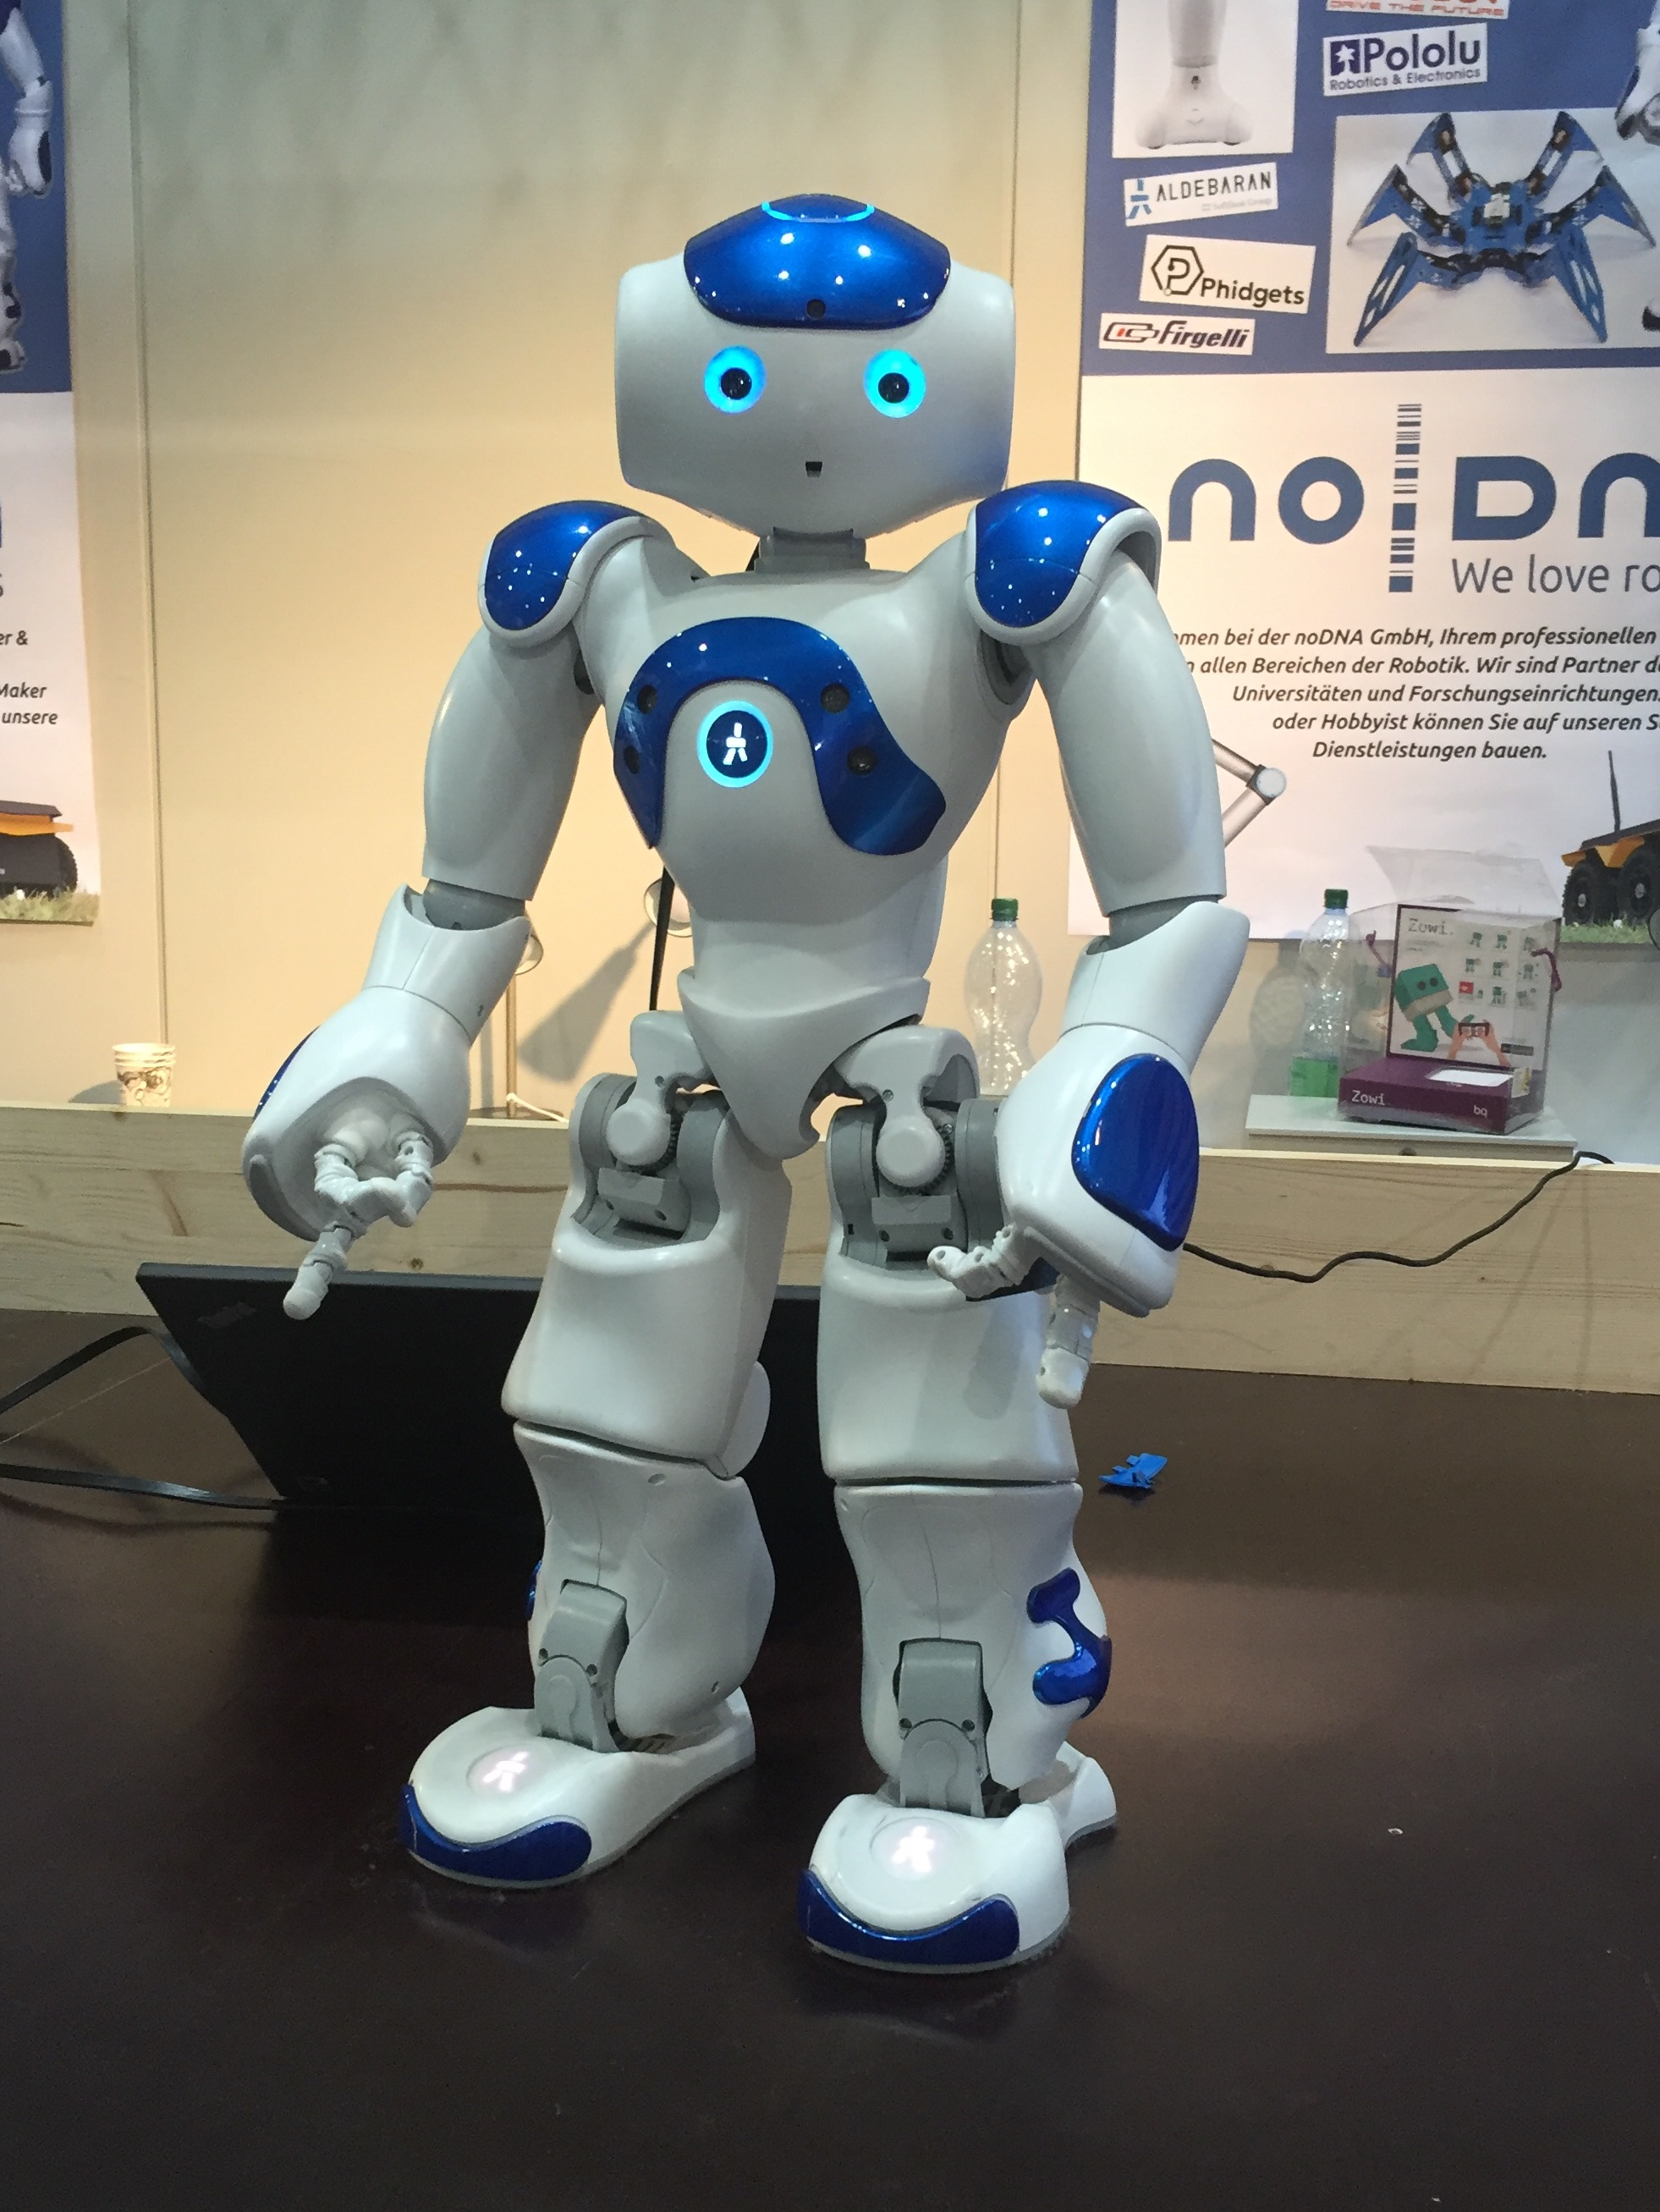
\includegraphics[width=5cm]{Images/nao_robot.jpg} % Used to add images to TEX documents, can accept parameters for dimensions. Input path is local.

% The following code can be used to make tables with set widths for a given column, by designating a capital justification letter and {<width>cm}
\newcolumntype{L}[1]{>{\raggedright\let\newline\\\arraybackslash\hspace{0pt}}m{#1}}
\newcolumntype{C}[1]{>{\centering\let\newline\\\arraybackslash\hspace{0pt}}m{#1}}
\newcolumntype{R}[1]{>{\raggedleft\let\newline\\\arraybackslash\hspace{0pt}}m{#1}}

Tabular example:

\begin{tabular}{|l|C{8cm}|r|} % Definition of a table. The parameters are letters, representing the alignments of each column, and the vertical lines representing separators (optional). Horizontal lines should be declared within the environment.
    \hline
    Left & Center & Right \\
    \hline
    A & B & C \\
    \hline
\end{tabular}

Matrix/Array example:

% Arrays must be explicitly defined within math mode ($$) and are worked with similarly to the tabular class.
$\left[\begin{array}{ccc}
    a_{1} & a_{2} & a_{3} \\
    a_{4} & a_{5} & a_{6}
\end{array}\right]$

This can also be done the AMS way:

$\begin{pmatrix}
    a_{1} & a_{2} & a_{3} & \cdots \\
    a_{4} & a_{5} & a_{6} & \cdots 
\end{pmatrix}$

\noindent\rule{\textwidth}{1pt}

\section{Calculus Notation}
Polynomials:
\(\displaystyle f(x) = a_n x^n + a^{n-1} x^{n-1} + \cdots + a_1 x + a_0\)

Exponentials:
\(\displaystyle c_1 e^{r_1 x} + c_2 e^{r_2 x} + \cdots + c_n e^{r_n x}\)

Limits:
\(\displaystyle \lim_{x \to \infty} \frac{x^2 + 1}{x^2 - 1} = 1\)

Summations:
\(\displaystyle \sum_{\substack{n=0 \\ n \text{ odd }}}^{\infty} a_{x} x^n\)

Integrals:
\(\displaystyle \int_0^{\infty} f(x) \, \differential{}\), \(\displaystyle \int_a^b f(x) \, dx = F(x) \bigg\vert_a^b\)

Derivatives:
\(\displaystyle \frac{df}{dx}\), \(\displaystyle f'(x)\)

Partial derivatives:
\(\displaystyle \frac{\partial f}{\partial x}\)

Vectors: 
\(\displaystyle \vv{r}(t) = \langle x(t), y(t), z(y) \rangle\)

Calc 3 Construct:
\(\displaystyle \oint \vv{e} \cdot d\vv{s} = \dfrac{d\Phi_B}{dt}\)

\noindent\rule{\textwidth}{1pt}

\section{Extra Math}
Square Root:
\(\sqrt{x}\), \(\sqrt[3]{\frac{x}{y}}\)

Quadratic Formula:
If \(ax^2 + bx + c = 0\) then 
\(\displaystyle x = \frac{-b \pm \sqrt{b^2 - 4ac}}{2a}\)

Set Theory:
\(\{x \in S \mid P(x)\}\), \(\{\forall x \exists a \mid a = x, \therefore x = x\}\)

Combinatorics:
\(\displaystyle \binom{n}{k}\), \({}_nC_k\), \({}_nP_k\)
\end{document} % Indicates the end of a document

